\documentclass[11pt]{article}

\usepackage[margin=1in]{geometry}
\usepackage{amsmath, amssymb}
\usepackage{graphicx}
\usepackage{booktabs}
\usepackage[hidelinks]{hyperref}
\usepackage{placeins}

\title{BUSFIN 8200: Problem Set 1}
\author{Xi Wang}
\date{\today}

\begin{document}

\maketitle

\section{Question 1}

\subsection{Part (a)}

Assume $D_t > 0$. By definition, the gross return on equity is
\begin{equation}
R_{e,t+1} = \frac{P_{t+1}+D_{t+1}}{P_t}.
\end{equation}
Taking logs,
\begin{align*}
\log(R_{e,t+1}) &= \log\!\left(\frac{P_{t+1}+D_{t+1}}{P_t}\right) \\
&= \log\!\left(\frac{P_{t+1}+D_{t+1}}{P_{t+1}}\cdot P_{t+1}\right) - \log(P_t) \\
&= \log\!\left[\left(1+\frac{D_{t+1}}{P_{t+1}}\right)P_{t+1}\right] - \log(P_t) \\
&= \log(P_{t+1}) + \log\!\left(1+\frac{D_{t+1}}{P_{t+1}}\right) - \log(P_t).
\end{align*}

Define $r_{e,t+1} \equiv \log(R_{e,t+1})$, $p_t \equiv \log(P_t)$, and $d_t \equiv \log(D_t)$.
Since $\dfrac{D_{t+1}}{P_{t+1}} = e^{\log(D_{t+1}/P_{t+1})} = e^{d_{t+1}-p_{t+1}}$, we can write
\[
r_{e,t+1} = p_{t+1} + \log\!\left(1+e^{d_{t+1}-p_{t+1}}\right) - p_t.
\]

Define $f(x) \equiv \log(1+e^{x})$, where $x = d_{t+1}-p_{t+1}$. We approximate this function
around the average log dividend-price ratio $\overline{d-p}$ using a first-order Taylor
approximation,
\[
f(x) \approx f(\overline{d-p}) + f'(\overline{d-p})\big(x-\overline{d-p}\big),
\]
so that
\[
f(d_{t+1}-p_{t+1}) \approx f(\overline{d-p}) + f'(\overline{d-p})\Big[(d_{t+1}-p_{t+1}) - \overline{d-p}\Big].
\]

Since $f(x) = \log(1+e^{x})$, we have $f'(x) = \dfrac{e^{x}}{1+e^{x}}$, so
\[
f'(\overline{d-p}) = \frac{e^{\overline{d-p}}}{1+e^{\overline{d-p}}}.
\]
Define $\kappa \equiv \dfrac{1}{1+e^{\overline{d-p}}}$. Then $1-\kappa = \dfrac{e^{\overline{d-p}}}{1+e^{\overline{d-p}}}$, so $f'(\overline{d-p}) = 1-\kappa$.

Hence,
\begin{align*}
f(d_{t+1}-p_{t+1}) &\approx f(\overline{d-p}) + (1-\kappa)\Big[(d_{t+1}-p_{t+1}) - \overline{d-p}\Big] \\
&= f(\overline{d-p}) - (1-\kappa)\overline{d-p} + (1-\kappa)(d_{t+1}-p_{t+1}).
\end{align*}

Define $\kappa_0 \equiv f(\overline{d-p}) - (1-\kappa)\overline{d-p}$, a constant. Since
$f(\overline{d-p}) = \log(1+e^{\overline{d-p}})$ and $\kappa = \dfrac{1}{1+e^{\overline{d-p}}}$,
we have $1+e^{\overline{d-p}} = \dfrac{1}{\kappa}$, so
\[
f(\overline{d-p}) = \log\!\left(\frac{1}{\kappa}\right) = -\log\kappa,
\qquad
e^{\overline{d-p}} = \frac{1}{\kappa}-1,
\qquad
\overline{d-p} = \log\!\left(\frac{1}{\kappa}-1\right).
\]
Therefore,
\[
\kappa_0 \equiv f(\overline{d-p}) - (1-\kappa)\overline{d-p} = -\log\kappa - (1-\kappa)\log\!\left(\frac{1}{\kappa}-1\right).
\]

We then have $\log(1+e^{d_{t+1}-p_{t+1}}) = f(d_{t+1}-p_{t+1}) \approx \kappa_0 + (1-\kappa)(d_{t+1}-p_{t+1})$, so
\begin{align*}
r_{e,t+1} &= p_{t+1} + \log\!\left(1+e^{d_{t+1}-p_{t+1}}\right) - p_t \\
&\approx p_{t+1} + \kappa_0 + (1-\kappa)(d_{t+1}-p_{t+1}) - p_t \\
&= \kappa_0 + (1-\kappa)d_{t+1} + \kappa p_{t+1} - p_t \\
&= \kappa_0 + \Big[(1-\kappa)d_{t+1} - d_t + \kappa p_{t+1} - p_t + d_t\Big] \\
&= \kappa_0 + (d_{t+1}-d_t) + \kappa(p_{t+1}-d_{t+1}) - (p_t-d_t) \\
&= \kappa_0 + \Delta d_{t+1} + \kappa(p_{t+1}-d_{t+1}) - (p_t-d_t).
\end{align*}

Therefore, we have
\begin{align*}
r_{e,t+1} &\approx \kappa_0 + \Delta d_{t+1}
    + \kappa(p_{t+1}-d_{t+1}) - (p_t-d_t), \\
\kappa &= \frac{1}{1+e^{\overline{d-p}}}, \\
\kappa_0 &= -\log(\kappa)
    - (1-\kappa)\log\!\left(\frac{1}{\kappa}-1\right).
\end{align*}

Isolating $p_t-d_t$ and recursively substituting for $p_{t+h}-d_{t+h}$, we have
\begin{align*}
(p_t - d_t) &\approx \kappa_0 - r_{e,t+1} + \Delta d_{t+1} + \kappa(p_{t+1}-d_{t+1}) \\
&= \kappa_0 - r_{e,t+1} + \Delta d_{t+1} + \kappa\Big[\kappa_0 - r_{e,t+2} + \Delta d_{t+2} + \kappa(p_{t+2}-d_{t+2})\Big] \\
&= (1+\kappa)\kappa_0 + (\Delta d_{t+1}+\kappa \Delta d_{t+2}) - (r_{e,t+1}+\kappa r_{e,t+2}) + \kappa^{2}(p_{t+2}-d_{t+2}) \\
&\ \ \vdots \quad \text{keep substituting } p_{t+h}-d_{t+h} \\
&= \frac{\kappa_0(1-\kappa^{H})}{1-\kappa} + \sum_{h=1}^{H}\kappa^{h-1}\Delta d_{t+h} - \sum_{h=1}^{H}\kappa^{h-1}r_{e,t+h} + \kappa^{H}(p_{t+H}-d_{t+H}).
\end{align*}

Thus, we have
\[
d_t - p_t \approx \frac{\kappa_0(\kappa^{H}-1)}{1-\kappa} + \sum_{h=1}^{H}\kappa^{h-1}r_{e,t+h} - \sum_{h=1}^{H}\kappa^{h-1}\Delta d_{t+h} + \kappa^{H}(d_{t+H}-p_{t+H}),
\]
so, letting $dp_t \equiv d_t - p_t$,
\begin{equation*}
dp_t \approx \frac{\kappa_0(\kappa^{H}-1)}{1-\kappa} + \sum_{h=1}^{H}\kappa^{h-1}r_{e,t+h} - \sum_{h=1}^{H}\kappa^{h-1}\Delta d_{t+h} + \kappa^{H} dp_{t+H}. \tag{1.1}
\end{equation*}

Taking expectations as of time $t$,
\begin{equation*}
dp_t = \frac{\kappa_0(\kappa^{H}-1)}{1-\kappa} + \sum_{h=1}^{H}\kappa^{h-1}\mathbb{E}_t[r_{e,t+h}] - \sum_{h=1}^{H}\kappa^{h-1}\mathbb{E}_t[\Delta d_{t+h}] + \kappa^{H}\mathbb{E}_t[dp_{t+H}]. \tag{1.2}
\end{equation*}

Suppose $H\to\infty$. Since $\kappa = \dfrac{1}{1+e^{\overline{d-p}}} \in (0,1)$, we have
$\lim_{H\to\infty}\kappa^{H}=0$, and by the no-bubble condition $\lim_{H\to\infty}\kappa^{H}\mathbb{E}_t[dp_{t+H}]=0$.
Therefore,
\begin{equation*}
dp_t = \frac{-\kappa_0}{1-\kappa} + \sum_{h=1}^{\infty}\kappa^{h-1}\mathbb{E}_t[r_{e,t+h}] - \sum_{h=1}^{\infty}\kappa^{h-1}\mathbb{E}_t[\Delta d_{t+h}]. \tag{1.3}
\end{equation*}

\subsection{Part (b)}
\begin{figure}[htbp]
    \centering
    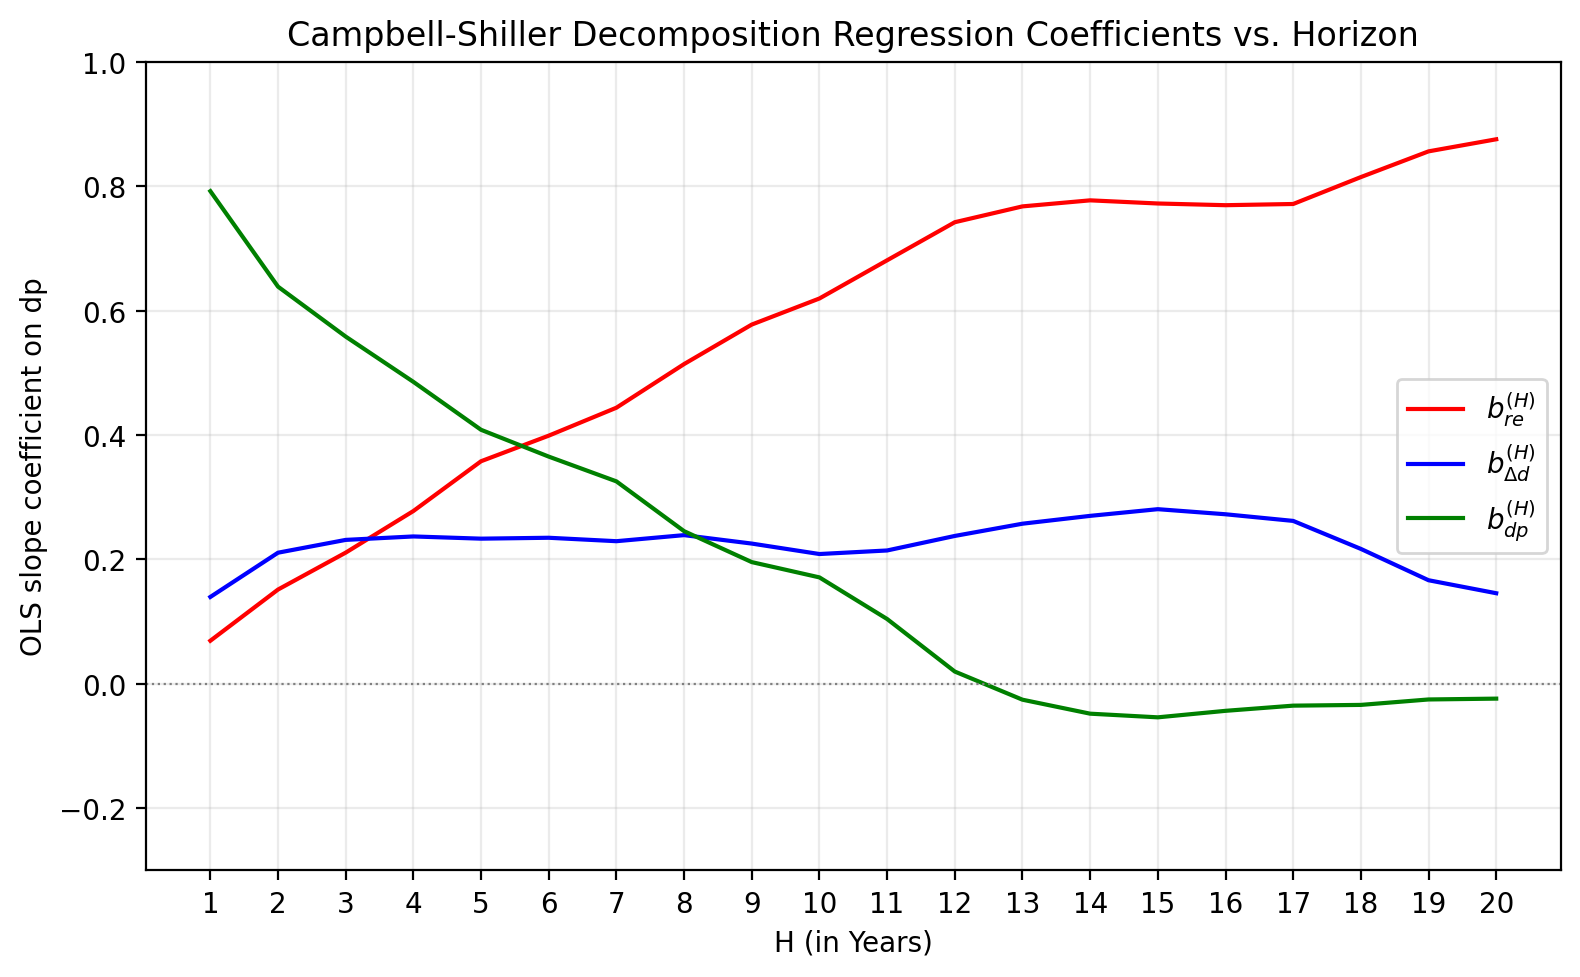
\includegraphics[width=0.8\textwidth]{figures/q1b_coefficients.png}
    \caption{OLS slope coefficients of \texttt{future\_return}, \texttt{change\_d}, and \texttt{dp\_H} on \texttt{dp}, plotted against the horizon $H$ (in years).}
    \label{fig:q1b_coefficients}
\end{figure}

From the equation
\[
1
=
\underbrace{
\frac{
\operatorname{Cov}\left[
dp_t,\,
\sum_{h=1}^{H}\kappa^{h-1} r_{e,t+h}
\right]
}{
\operatorname{Var}[dp]
}
}_{b_{r_e}^{(H)}}
+
\underbrace{
\frac{
\operatorname{Cov}\left[
dp_t,\,
-\sum_{h=1}^{H}\kappa^{h-1}\Delta d_{t+h}
\right]
}{
\operatorname{Var}[dp]
}
}_{b_{\Delta d}^{(H)}}
+
\underbrace{
\frac{
\operatorname{Cov}\left[
dp_t,\,
\kappa^H dp_{t+H}
\right]
}{
\operatorname{Var}[dp]
}
}_{b_{dp}^{(H)}}.
\]

This equation is trying to measure, how much each component moves when today's $dp_{t}$ moves. The meaning of these three coefficients is as follows:

\[
\sum_{h=1}^{H}\kappa^{h-1}\mathbb{E}_t[r_{e,t+h}] = a + b_{r_e}^{(H)} dp_t + \epsilon_t
\]

The slope is $b_{r_e}^{(H)}$, and it measures the sensitivity of expected discounted future returns to today's dividend-price ratio.

Because dividend growth enters the Campbell–Shiller equation with a minus sign, define
\[
-\sum_{h=1}^{H}\kappa^{h-1} \mathbb{E}_t [\Delta d_{t+h} ]=a+b_{\Delta d}^{(H)} dp_t+\epsilon_t.
\]

So $b_{\Delta d}^{(H)}$ captures how much variation in $dp_t$ is associated with expected future dividend growth.

\[
\kappa^H \mathbb{E}_t [dp_{t+H} ]=a+b_{dp}^{(H)} dp_t+\epsilon_t.
\] 

$b_{dp}^{(H)}$ tells us how much today's high $dp_{t}$ is simply expected to persist into the future.

\[
1 = b_{r_e}^{(H)} + b_{\Delta d}^{(H)} + b_{dp}^{(H)}
\]

From the graph, we can see that the contributions of expected future returns, expected future dividend growth, and the future dividend-price ratio to the variation in today's $dp_{t}$ change with the horizon $H$.
In the short run, the variation in today's $dp_{t}$ is primarily driven by the future dividend-price ratio. As the horizon $H$ increases, the contribution of expected future returns becomes more significant, while the contribution of the future dividend-price ratio declines toward zero. The contribution of negative expected future dividend growth remains relatively stable across different horizons.
Also, if we add up these three coefficients, we get approximately 1, which reflects the normalized variance decomposition of today's $dp_{t}$.

% TODO: discussion of the figure and results

\subsection{Part (c)}
\FloatBarrier
\begin{figure}[htbp]
    \centering
    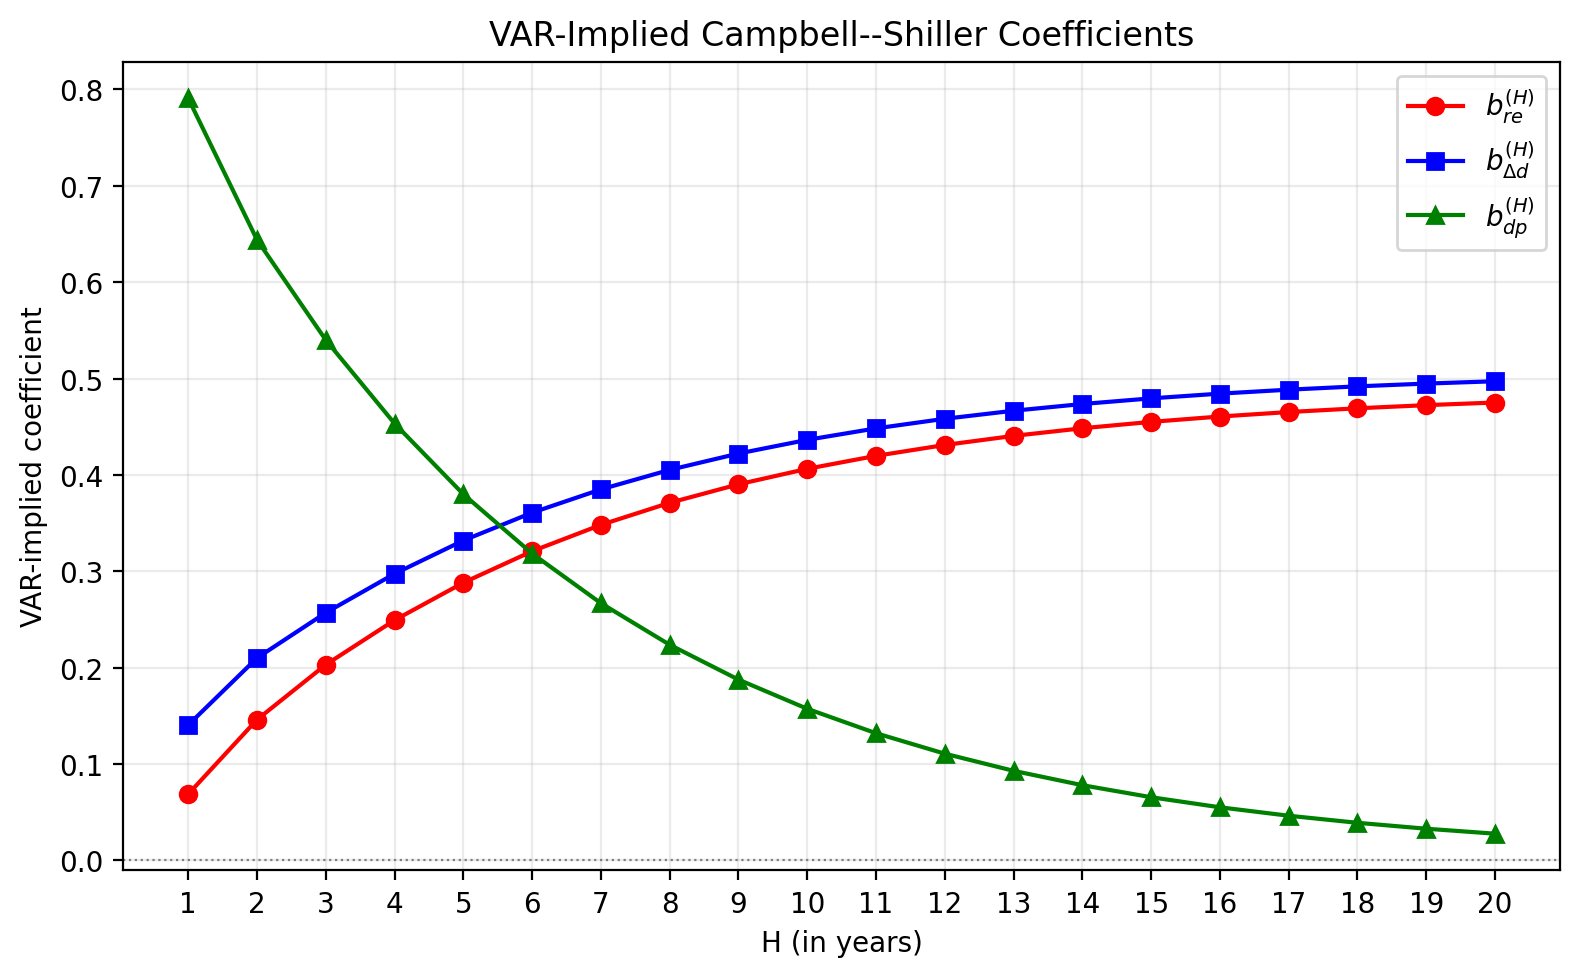
\includegraphics[width=0.8\textwidth]{figures/q1c_var_implied_coefficients.png}
    \caption{VAR-implied coefficients}
    \label{fig:q1c_var_implied_coefficients}
\end{figure}
\FloatBarrier


The VAR-implied coefficients shown in Figure~\ref{fig:q1c_var_implied_coefficients} show some interesting patterns. Instead of the expected future return component alone becoming dominant as $H$ increases, the figure shows that both the expected future return component and the negative expected future dividend growth component contribute significantly to the variation in today's $dp_t$ across different horizons. At the same time, the contribution of the future dividend-price ratio declines as the horizon increases, consistent with the findings from the direct-regression estimates, although the decline appears to be more gradual under the VAR approach.
The difference in these patterns may arise because the two approaches estimate long-horizon coefficients differently. The direct approach estimates each horizon separately using realized future outcomes, whereas the VAR approach estimates the joint one-year dynamics of the state variables and uses the estimated transition matrix to imply coefficients at all subsequent horizons.

\subsection{Part (d)}
The resulting long-run VAR-implied coefficients are reported in Table~\ref{tab:q1d_long_run}. The table shows that, in the long run, the contributions of expected future returns and negative expected future dividend growth are roughly equal, accounting for approximately 49\% and 51\%, respectively. Their sum is 0.998808, which is close to, but not exactly, one. This indicates that the unrestricted estimated VAR approximately, rather than mechanically, satisfies the long-run Campbell--Shiller restriction.
\begin{table}[htbp]
    \centering
    \caption{Long-run VAR-implied coefficients}
    \label{tab:q1d_long_run}
    \begin{tabular}{lcc}
        \toprule
        Component & Coefficient & Estimate \\
        \midrule
        Expected return & $b_{re}^{(\infty)}$ & 0.489191 \\
        Negative expected dividend growth & $b_{dg}^{(\infty)}$ & 0.509617 \\
        Sum & $b_{re}^{(\infty)}+b_{dg}^{(\infty)}$ & 0.998808 \\
        \bottomrule
    \end{tabular}
\end{table}
\FloatBarrier

\subsection{Part (e)}

First, assume $D_t>0$. We have
\[
R_{e,t+1}=\frac{P_{t+1}+D_{t+1}}{P_t}.
\]
Then,
\begin{align*}
R_{e,t+1}\frac{D_t}{D_{t+1}}
&=\frac{P_{t+1}+D_{t+1}}{P_t}\frac{D_t}{D_{t+1}} \\
&=\frac{D_t}{P_t}\frac{P_{t+1}+D_{t+1}}{D_{t+1}} \\
&=\frac{
\dfrac{P_t+D_t}{P_t}\dfrac{D_t}{P_t+D_t}
}{
\dfrac{D_{t+1}}{P_{t+1}+D_{t+1}}
}.
\end{align*}

Taking logs on both sides gives
\begin{align*}
\log(R_{e,t+1})+\log\!\left(\frac{D_t}{D_{t+1}}\right)
&=\log\!\left(\frac{P_t+D_t}{P_t}\right)
+\log\!\left(\frac{D_t}{P_t+D_t}\right) \\
&\quad-\log\!\left(\frac{D_{t+1}}{P_{t+1}+D_{t+1}}\right).
\end{align*}

Define
\[
r_{e,t+1}=\log(R_{e,t+1}),
\qquad p_t=\log(P_t),
\qquad d_t=\log(D_t),
\qquad dy_t=\log\!\left(1+\frac{D_t}{P_t}\right).
\]
Given that
\begin{align*}
\log\!\left(\frac{D_t}{P_t+D_t}\right)
&=\log\!\left(1-\frac{P_t}{P_t+D_t}\right) \\
&=\log\!\left(1-e^{\log(P_t/(P_t+D_t))}\right) \\
&=\log\!\left(1-e^{-\log((P_t+D_t)/P_t)}\right) \\
&=\log\!\left(1-e^{-\log(1+D_t/P_t)}\right) \\
&=\log\!\left(1-e^{-dy_t}\right),
\end{align*}
we have
\[
\log\!\left(\frac{D_t}{P_t+D_t}\right)
=\log\!\left(1-e^{-dy_t}\right).
\]
Similarly,
\[
\log\!\left(\frac{D_{t+1}}{P_{t+1}+D_{t+1}}\right)
=\log\!\left(1-e^{-dy_{t+1}}\right).
\]
Therefore,
\[
r_{e,t+1}-\Delta d_{t+1}
=dy_t+\log\!\left(1-e^{-dy_t}\right)
-\log\!\left(1-e^{-dy_{t+1}}\right).
\]

Let
\[
f(x)=\log(1-e^{-x}).
\]
Then,
\[
f'(x)=\frac{1}{1-e^{-x}}e^{-x}
=\frac{e^{-x}}{1-e^{-x}}.
\]
Let $x=dy_t$. By a first-order approximation, and defining
$\kappa\equiv e^{-\overline{dy}}$, we have
\begin{align*}
\log\!\left(1-e^{-dy_t}\right)
&\approx \log\!\left(1-e^{-\overline{dy}}\right)
+\log'\!\left(1-e^{-\overline{dy}}\right)(dy_t-\overline{dy}) \\
&=\log(1-\kappa)
+\frac{e^{-\overline{dy}}}{1-e^{-\overline{dy}}}
(dy_t-\overline{dy}) \\
&=\log(1-\kappa)+\frac{\kappa}{1-\kappa}
(dy_t-\overline{dy}).
\end{align*}
Thus,
\[
\log\!\left(1-e^{-dy_t}\right)
\approx \log(1-\kappa)+\frac{\kappa}{1-\kappa}
(dy_t-\overline{dy}).
\]
Similarly,
\[
\log\!\left(1-e^{-dy_{t+1}}\right)
\approx \log(1-\kappa)+\frac{\kappa}{1-\kappa}
(dy_{t+1}-\overline{dy}).
\]

Substituting these approximations into
$r_{e,t+1}-\Delta d_{t+1}
=dy_t+\log(1-e^{-dy_t})-\log(1-e^{-dy_{t+1}})$, we obtain
\begin{align*}
r_{e,t+1}-\Delta d_{t+1}
&=dy_t+\log(1-\kappa)
+\frac{\kappa}{1-\kappa}(dy_t-\overline{dy}) \\
&\quad-\log(1-\kappa)
-\frac{\kappa}{1-\kappa}(dy_{t+1}-\overline{dy}) \\
&=dy_t+\frac{\kappa}{1-\kappa}(dy_t-dy_{t+1}) \\
&=\frac{1}{1-\kappa}dy_t
-\frac{\kappa}{1-\kappa}dy_{t+1}.
\end{align*}
Therefore,
\begin{align*}
\frac{1}{1-\kappa}dy_t
&=r_{e,t+1}-\Delta d_{t+1}
+\frac{\kappa}{1-\kappa}dy_{t+1}, \\
dy_t
&=(1-\kappa)(r_{e,t+1}-\Delta d_{t+1})
+\kappa dy_{t+1}.
\end{align*}

Recursively substituting for future values of $dy$, we have
\begin{align*}
dy_t
&=(1-\kappa)(r_{e,t+1}-\Delta d_{t+1}) \\
&\quad+\kappa\left[(1-\kappa)(r_{e,t+2}-\Delta d_{t+2})
+\kappa dy_{t+2}\right] \\
&\quad\vdots \qquad \text{keep substituting }dy_{t+h} \\
&=(1-\kappa)\left(
\sum_{h=1}^{H}\kappa^{h-1}r_{e,t+h}
-\sum_{h=1}^{H}\kappa^{h-1}\Delta d_{t+h}
\right)+\kappa^Hdy_{t+H}.
\end{align*}
Thus, we have
\[
dy_t=(1-\kappa)\left(
\sum_{h=1}^{H}\kappa^{h-1}r_{e,t+h}
-\sum_{h=1}^{H}\kappa^{h-1}\Delta d_{t+h}
\right)+\kappa^Hdy_{t+H}.
\]

Taking expectations at time $t$, we have
\[
dy_t=(1-\kappa)\left(
\sum_{h=1}^{H}\kappa^{h-1}\mathbb{E}_t[r_{e,t+h}]
-\sum_{h=1}^{H}\kappa^{h-1}\mathbb{E}_t[\Delta d_{t+h}]
\right)+\kappa^H\mathbb{E}_t[dy_{t+H}].
\]

Suppose $H\to\infty$. Given that
$\kappa=e^{-\overline{dy}}\in(0,1)$, we have
\[
\lim_{H\to\infty}\kappa^H=0.
\]
Also, because of the no-bubble condition,
\[
\lim_{H\to\infty}\kappa^H\mathbb{E}_t[dy_{t+H}]=0.
\]
Therefore,
\[
dy_t=(1-\kappa)\left(
\sum_{h=1}^{H}\kappa^{h-1}\mathbb{E}_t[r_{e,t+h}]
-\sum_{h=1}^{H}\kappa^{h-1}\mathbb{E}_t[\Delta d_{t+h}]
\right).
\]

\section{Question 2}

\subsection{Part (a)}
Figure~\ref{fig:q2a_adjusted_r2} shows that the adjusted $R^2$ generally rises
with the horizon, from about 4.6\% at one year to a peak of about 44.3\% at 14
years, before declining slightly to about 42.1\% at 15 years. Thus, the current
dividend-price ratio has substantially greater explanatory power for long-horizon
average excess returns than for one-year-ahead excess returns. 

\FloatBarrier
\begin{figure}[htbp]
    \centering
    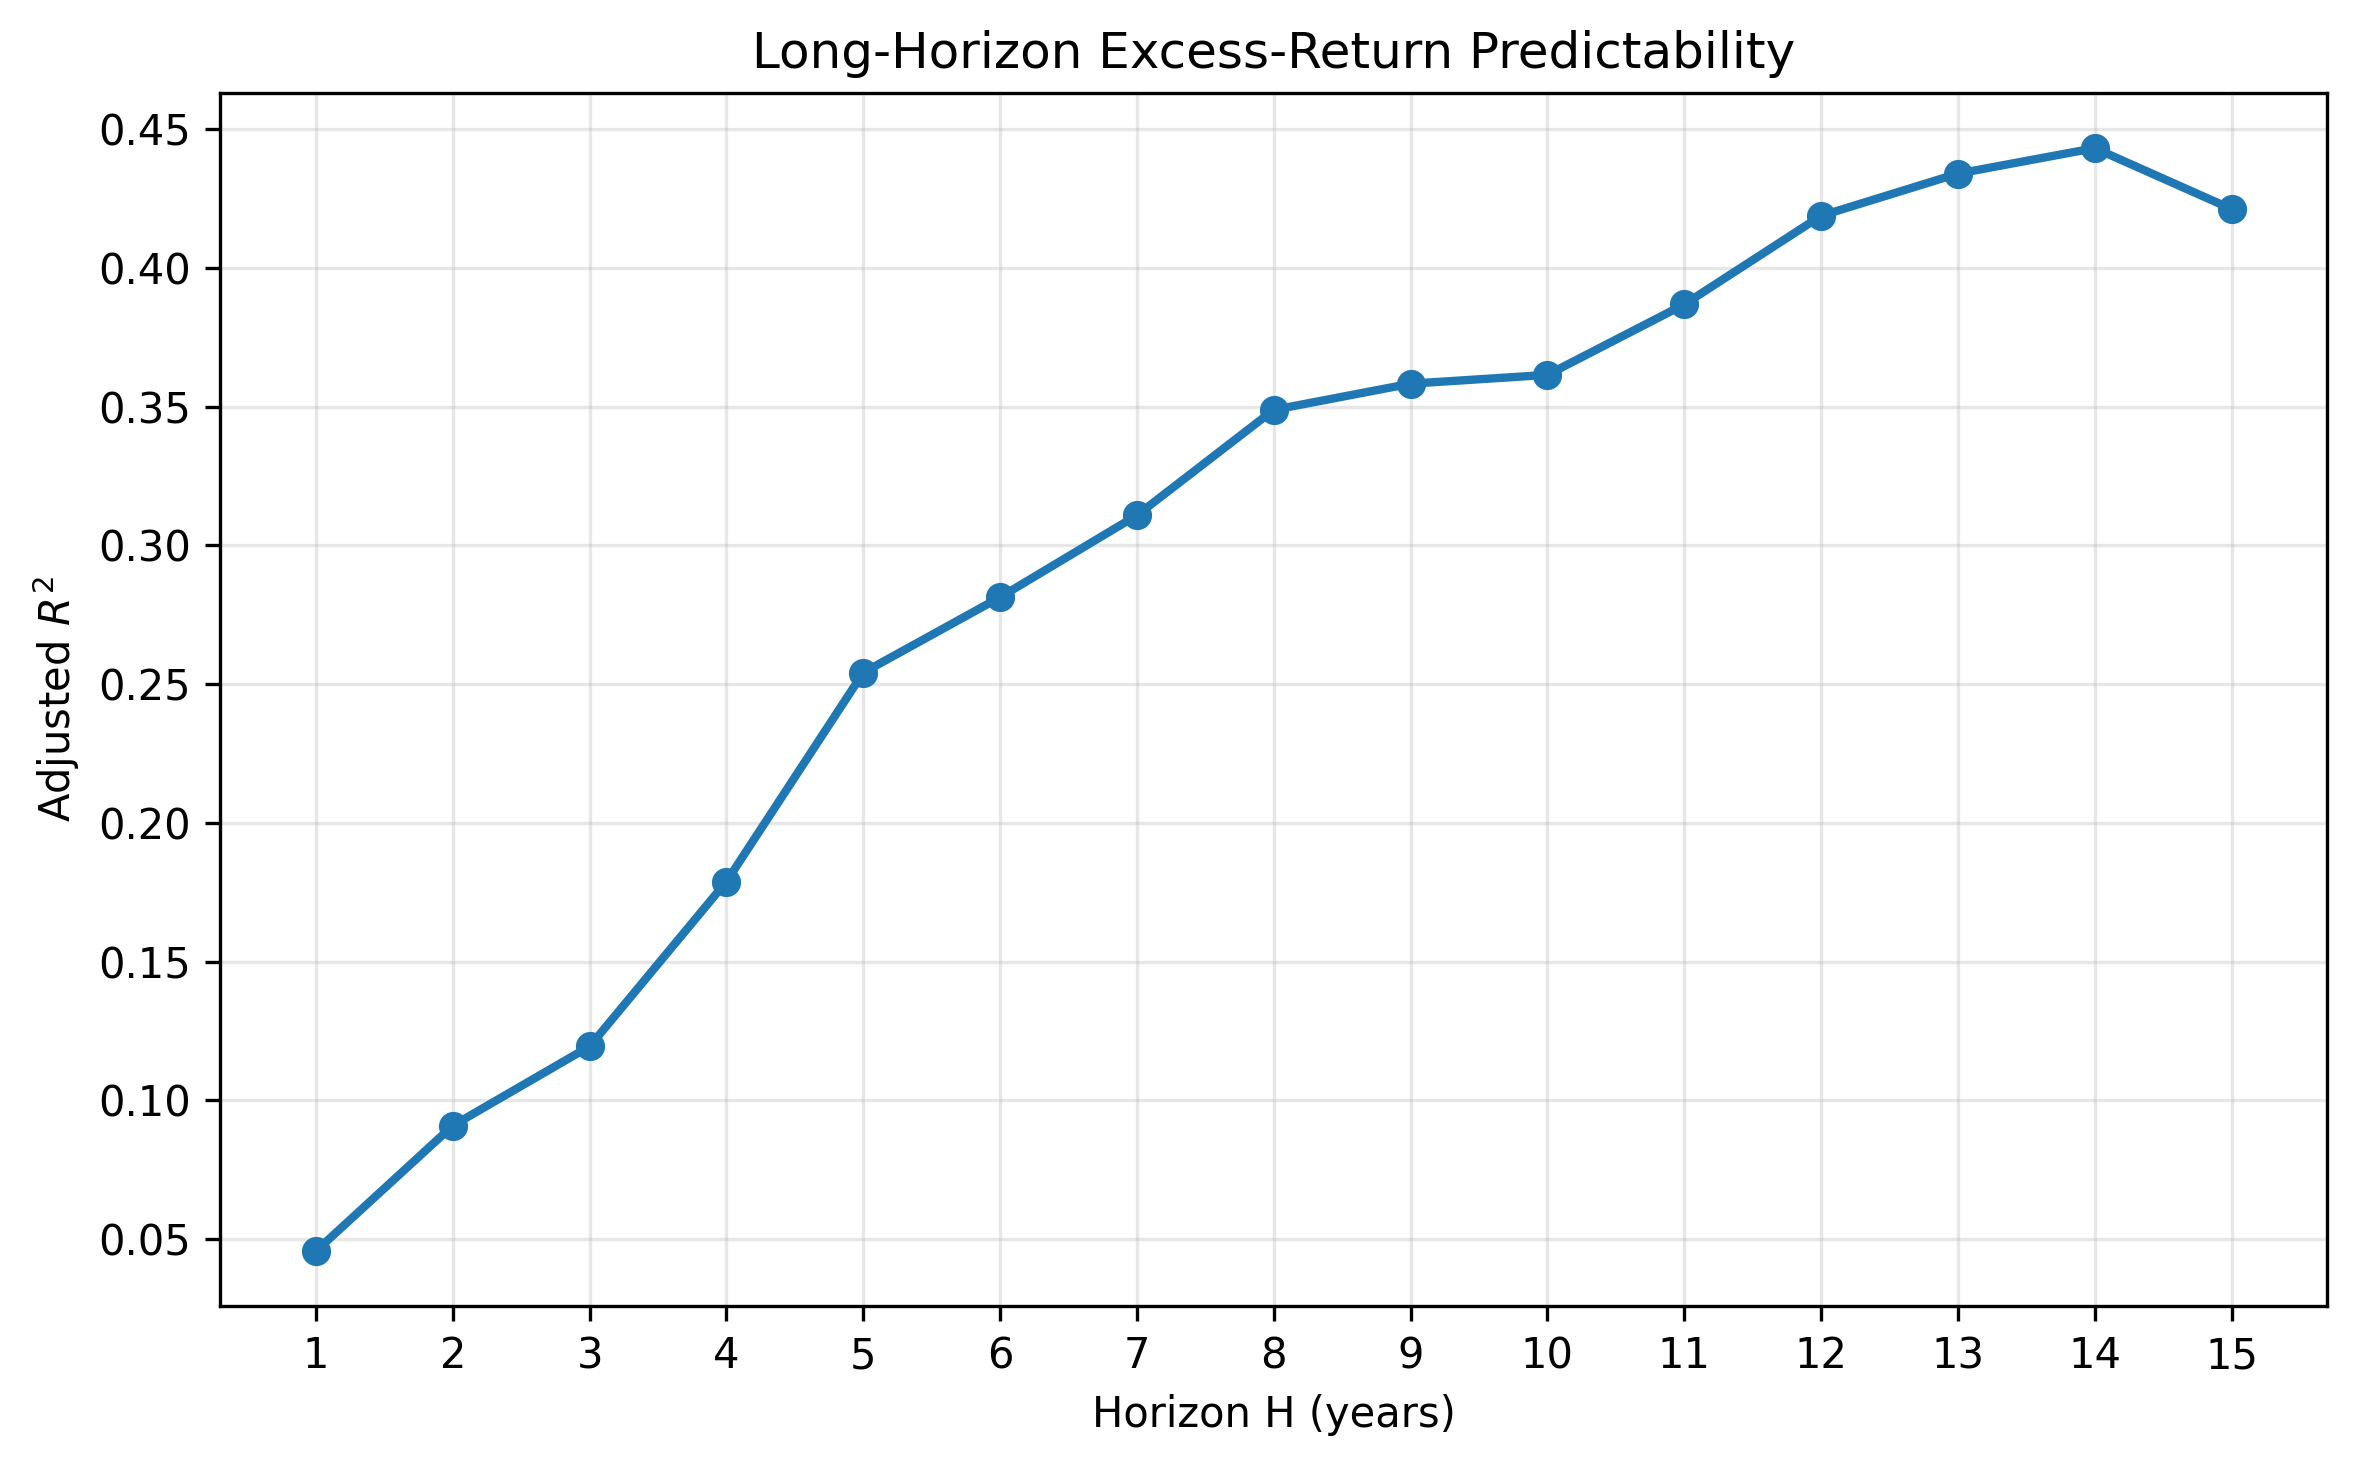
\includegraphics[width=0.8\textwidth]{figures/q2a_adjusted_r2.png}
    \caption{Adjusted $R^2$ from predictive regressions of average future annual
    simple excess returns on the starting dividend-price ratio.}
    \label{fig:q2a_adjusted_r2}
\end{figure}
\FloatBarrier

\clearpage
\subsection{Part (b)}

\begin{table}[htbp]
    \centering
    \caption{Q2(b) slope estimate and alternative standard errors}
    \label{tab:q2b_standard_errors}
    \begin{tabular}{lcccc}
        \toprule
        Method & $\widehat b$ & SE$(\widehat b)$ & $t$-statistic & Lags/bandwidth \\
        \midrule
        Baseline OLS & 2.8038 & 0.3802 & 7.3754 & 0 \\
        White (HC0) & 2.8038 & 0.6587 & 4.2569 & 0 \\
        Newey--West (1987) & 2.8038 & 1.2990 & 2.1584 & 11 \\
        Hansen--Hodrick (1980) & 2.8038 & 1.4537 & 1.9287 & 11 \\
        Newey--West (1994), automatic & 2.8038 & 1.2523 & 2.2390 & 22.0776 ($L=22$) \\
        \bottomrule
    \end{tabular}
\end{table}
\clearpage

\subsection{Part (c)}
From Table~\ref{tab:q2c_ah_estimates}, the Amihud and Hurvich estimate of $b$ is 2.3412, which is smaller than the
standard OLS estimate of 2.8038. It is natural for the two
estimates to differ because as
indicated by the estimated persistence coefficient $\widehat{\phi}=0.7197$, the predictor $D_t/P_t$ is persistent.
In a finite sample, persistence in the predictor can induce small-sample
bias in the OLS estimate of the predictive-regression coefficient.
The Amihud and Hurvich procedure corrects for this problem by first
bias-correcting the persistence coefficient from $\widehat{\phi}=0.7197$
to $\widehat{\phi}^{c}=0.7540$ and then including the resulting
bias-corrected residual $\widehat{u}^{c}_{t+1}$ in the predictive regression.
Thus, the difference between $\widehat b_{\mathrm{AH}}$ and $\widehat b_{\mathrm{OLS}}$ is expected.

\begin{table}[htbp]
    \centering
    \caption{Q2(c) Amihud--Hurvich estimates}
    \label{tab:q2c_ah_estimates}
    \begin{tabular}{lc}
        \toprule
        Quantity & Estimate \\
        \midrule
        $\widehat\theta$ & 0.0111 \\
        $\widehat\phi$ & 0.7197 \\
        $T$ (years) & 95 \\
        $\widehat\phi^{c}$ & 0.7540 \\
        $\widehat b_{\mathrm{AH}}$ & 2.3412 \\
        $\widehat b_u$ & $-13.4837$ \\
        $\widehat b_{\mathrm{OLS}}$ & 2.8038 \\
        $\widehat b_{\mathrm{AH}}-\widehat b_{\mathrm{OLS}}$ & $-0.4626$ \\
        Observations & 1,117 \\
        \bottomrule
    \end{tabular}
\end{table}
\clearpage

\subsection{Part (d)}
I estimate Equation (2.2) out of sample using an expanding window. The first out-of-sample forecast corresponds to December 1940, using the dividend-price ratio observed in December 1939. 
At each forecast date, I re-estimate the predictive regression using the historical information available at that date and use the resulting coefficients to construct the out-of-sample forecast. 
I also calculate the historical expanding-window mean excess return, $\overline{xR}_{e,t}$, which serves as the benchmark forecast. 
The in-sample fitted values are obtained from the full-sample regression in Equation (2.2).

The out-of-sample $R^2$ is calculated as
$$
R^2_{OS}=1-\frac{\sum_t\left(xR_{e,t+1}-\widehat E_t^{OS}[xR_e]\right)^2}{\sum_t\left(xR_{e,t+1}-\overline{xR}_{e,t}\right)^2}.
$$

The $R^2_{OS}$ compares the forecast errors from the predictive regression with those from the historical expanding-window mean benchmark. A positive $R^2_{OS}$ indicates that the dividend-price-ratio forecast has a lower sum of squared forecast errors than the historical-mean forecast, whereas a negative value indicates that the historical mean performs better.

For the full out-of-sample period, I obtain $R^2_{OS}=-0.0061$. Thus, over the full evaluation period, the dividend-price-ratio forecast performs slightly worse than the historical-mean benchmark.

To examine variation in forecasting performance over time, I also calculate $R^2_{OS}$ using a 50-year (600-month) rolling window of forecast errors. The coefficients $a_\tau$ and $b_\tau$ continue to be estimated using the expanding window. Thus, the 50-year rolling window changes only the forecast errors included in the calculation of $R^2_{OS}$; it does not change how the forecasts themselves are constructed.

Figure \ref{fig:q2d_rolling_r2_os} shows substantial variation in out-of-sample forecasting performance over time. The rolling $R^2_{OS}$ is strongly positive in the early part of the sample, indicating that the dividend-price-ratio forecast outperforms the historical-mean benchmark over those 50-year windows. 
It subsequently declines and fluctuates around zero for much of the later sample, before becoming increasingly negative toward the end. 

\begin{figure}[htbp]
    \centering
    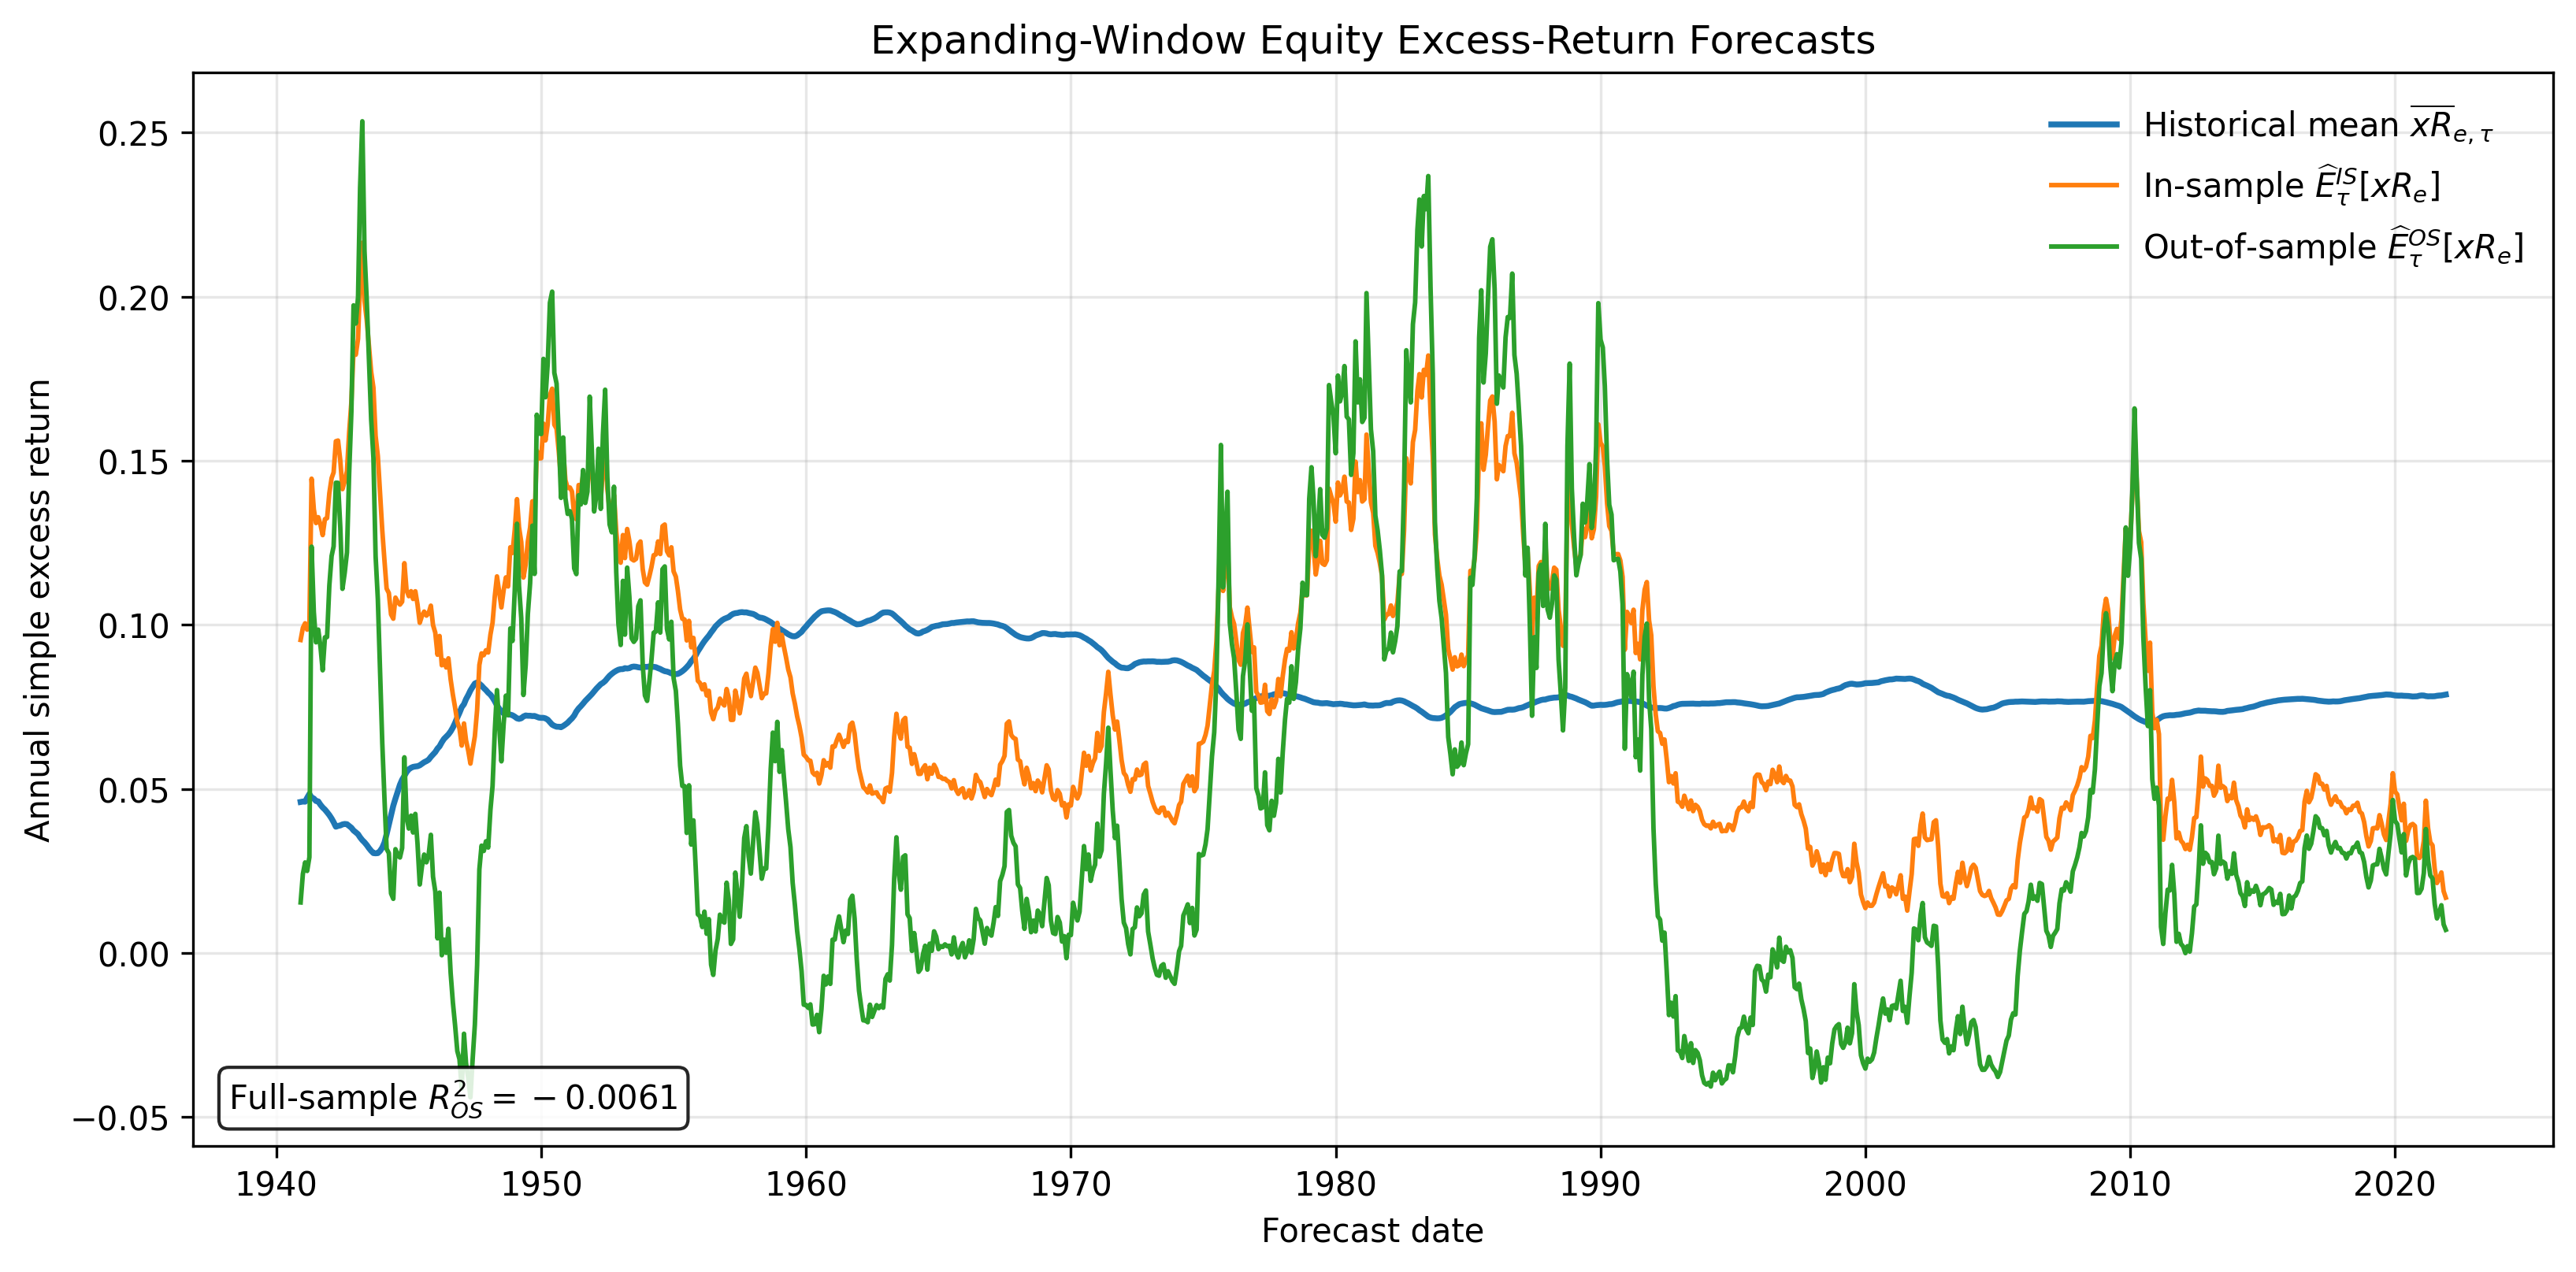
\includegraphics[width=0.9\textwidth]{figures/q2d_forecasts.png}
    \caption{Historical-mean, in-sample, and expanding-window out-of-sample
    forecasts of the annual simple equity excess return.}
    \label{fig:q2d_forecasts}
\end{figure}
\FloatBarrier

\begin{figure}[htbp]
    \centering
    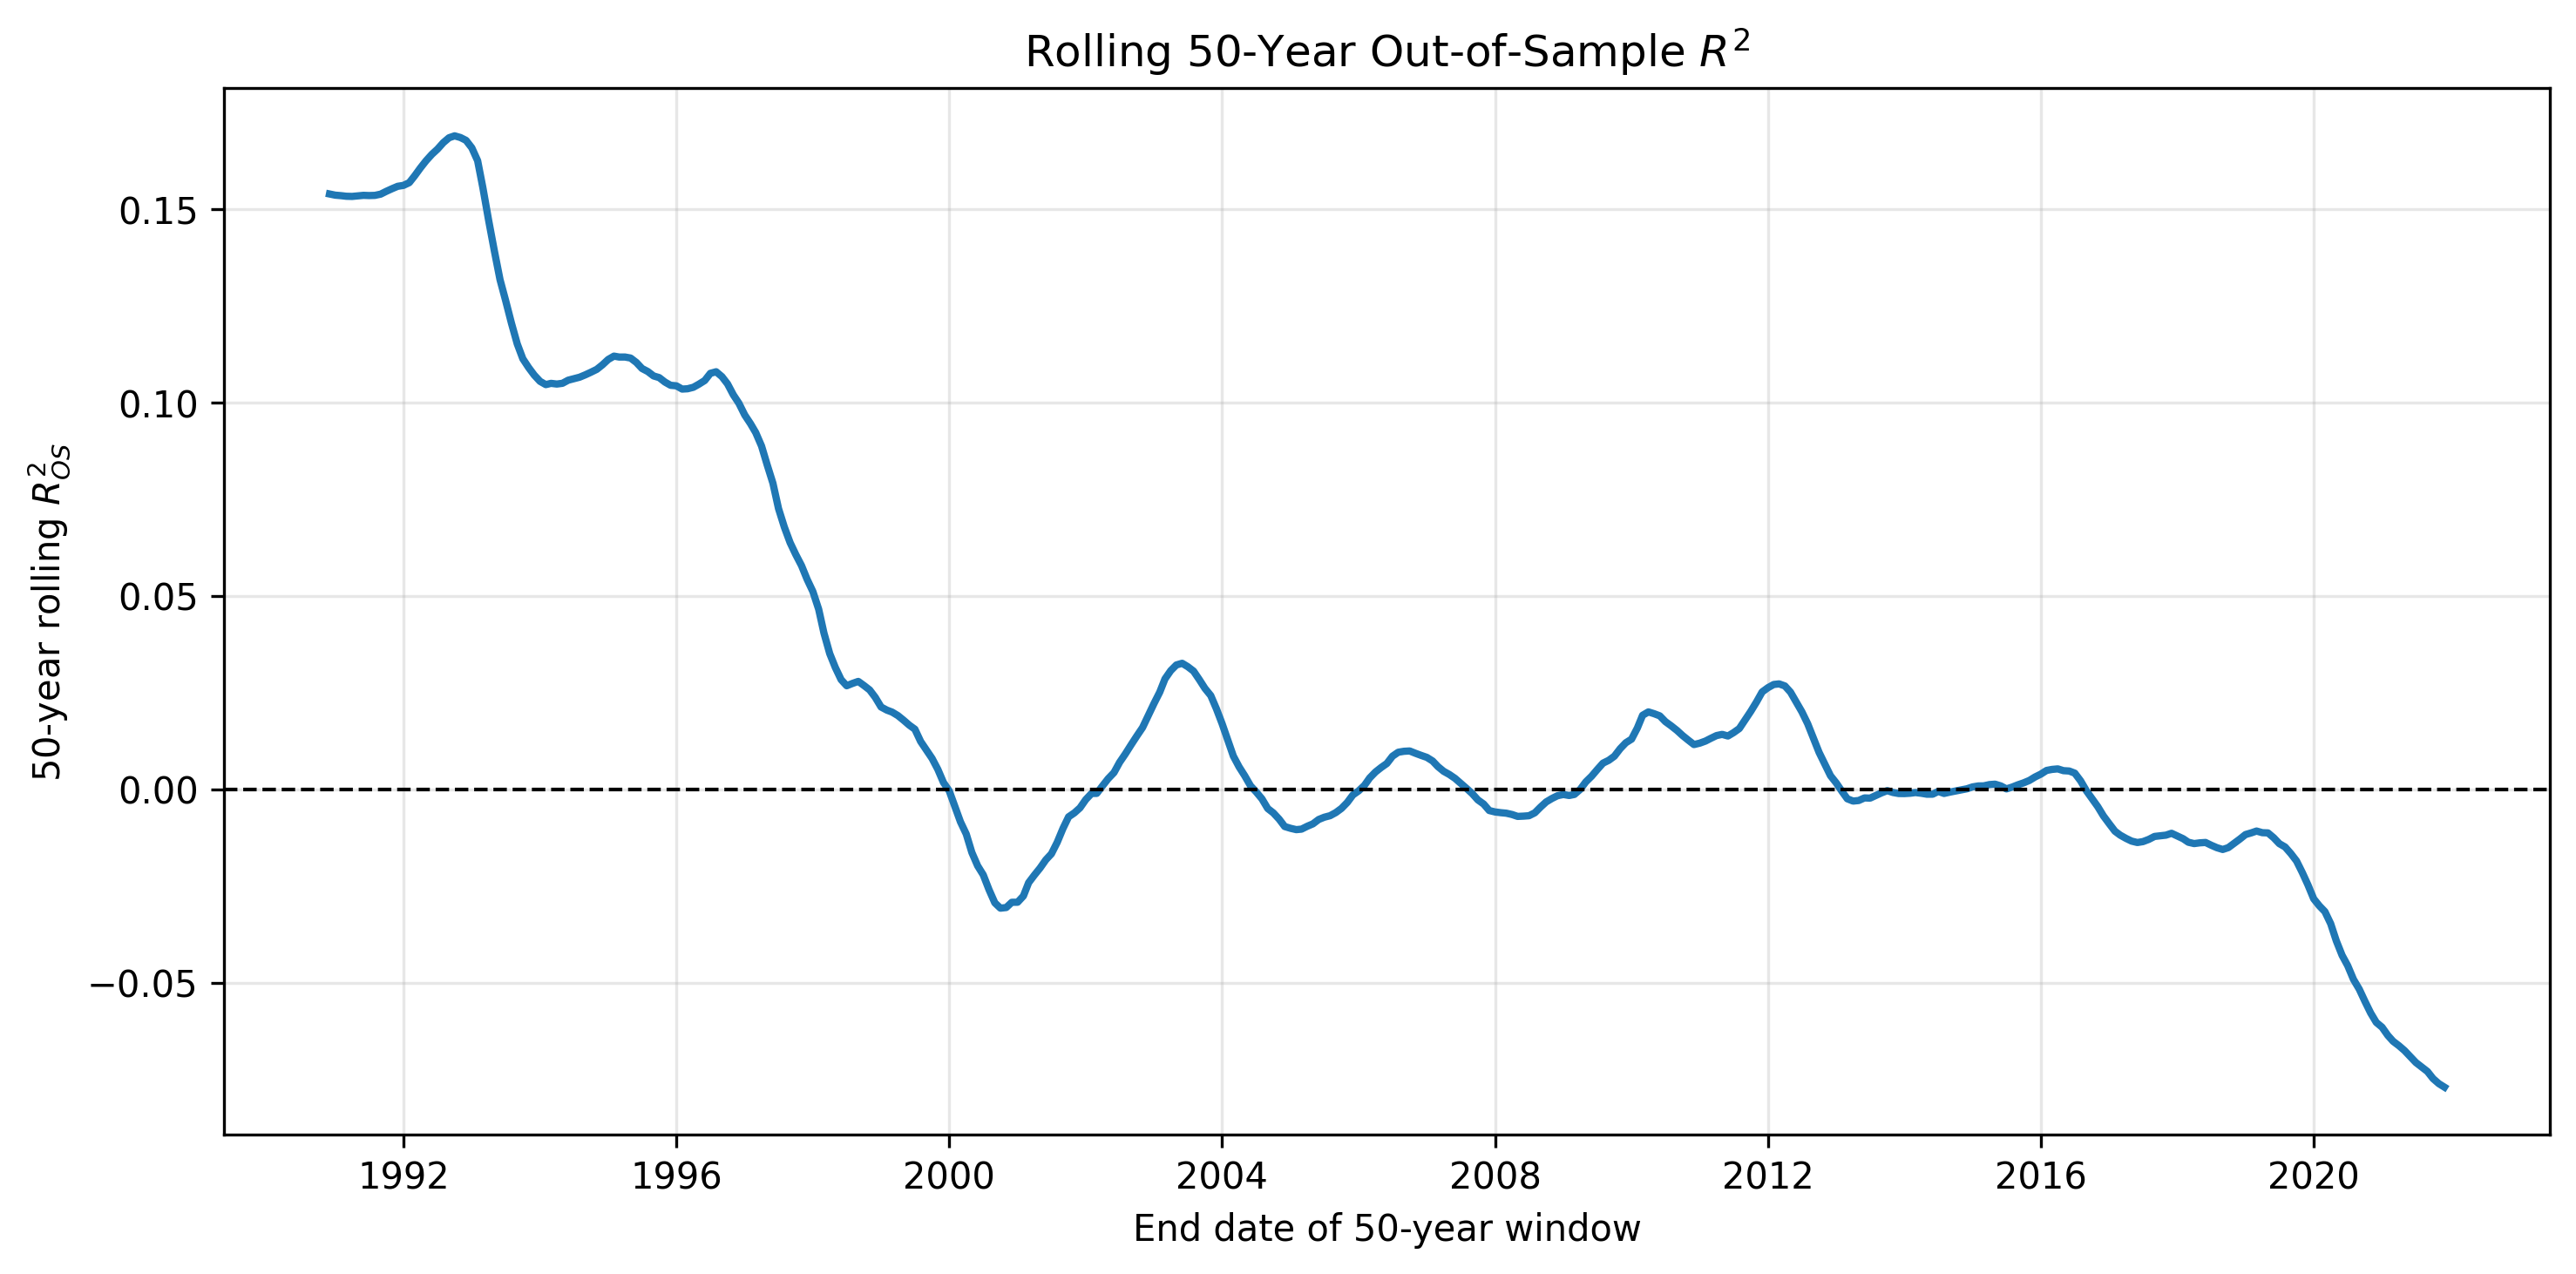
\includegraphics[width=0.9\textwidth]{figures/q2d_rolling_r2_os.png}
    \caption{Fifty-year rolling out-of-sample $R^2$.}
    \label{fig:q2d_rolling_r2_os}
\end{figure}
\FloatBarrier
\clearpage

\subsection{Part (e)}

I repeat the out-of-sample exercise in Part (d), but impose the steady-state
restrictions on the forecasting coefficients. For each forecast date $\tau$, I
calculate

\[
G_\tau = \operatorname{mean}\left(e^{dg_s}\right)
\]

using the same expanding historical sample used to calculate the historical-mean
forecast $\overline{xR}_{e,\tau}$. I then impose

\[
\widehat a_\tau = G_\tau-1,
\qquad
\widehat b_\tau = G_\tau,
\]

so that the restricted out-of-sample forecast is

\[
\widehat E_\tau^{OS}[xR_e]
=
(G_\tau-1)+G_\tau DP_\tau.
\]

Thus, unlike Part (d), the coefficients are not estimated by OLS at each forecast
date; instead, they are determined by the steady-state valuation restrictions.

Figure \ref{fig:q2e_restricted_forecasts} compares the restricted out-of-sample forecast with the historical-mean
forecast and the full-sample in-sample fitted values. Over the full out-of-sample
evaluation period, the restricted forecast produces

\[
R^2_{OS}=0.0321.
\]

Since this value is positive, the restricted steady-state forecast has a lower
sum of squared forecast errors than the historical-mean benchmark over the full
out-of-sample period.

Figure \ref{fig:q2e_rolling_r2_os} reports the 50-year rolling $R^2_{OS}$. As in Part (d), the rolling
window is applied only to the forecast errors used to calculate $R^2_{OS}$;
$G_\tau$ continues to be calculated using the expanding historical window.
The rolling $R^2_{OS}$ remains positive throughout the plotted period, indicating
that the restricted forecast outperforms the historical-mean benchmark over each
of these 50-year evaluation windows. However, its magnitude varies over time and
declines substantially toward the end of the sample, indicating that the degree
of out-of-sample improvement is not constant over time.

\begin{figure}[htbp]
    \centering
    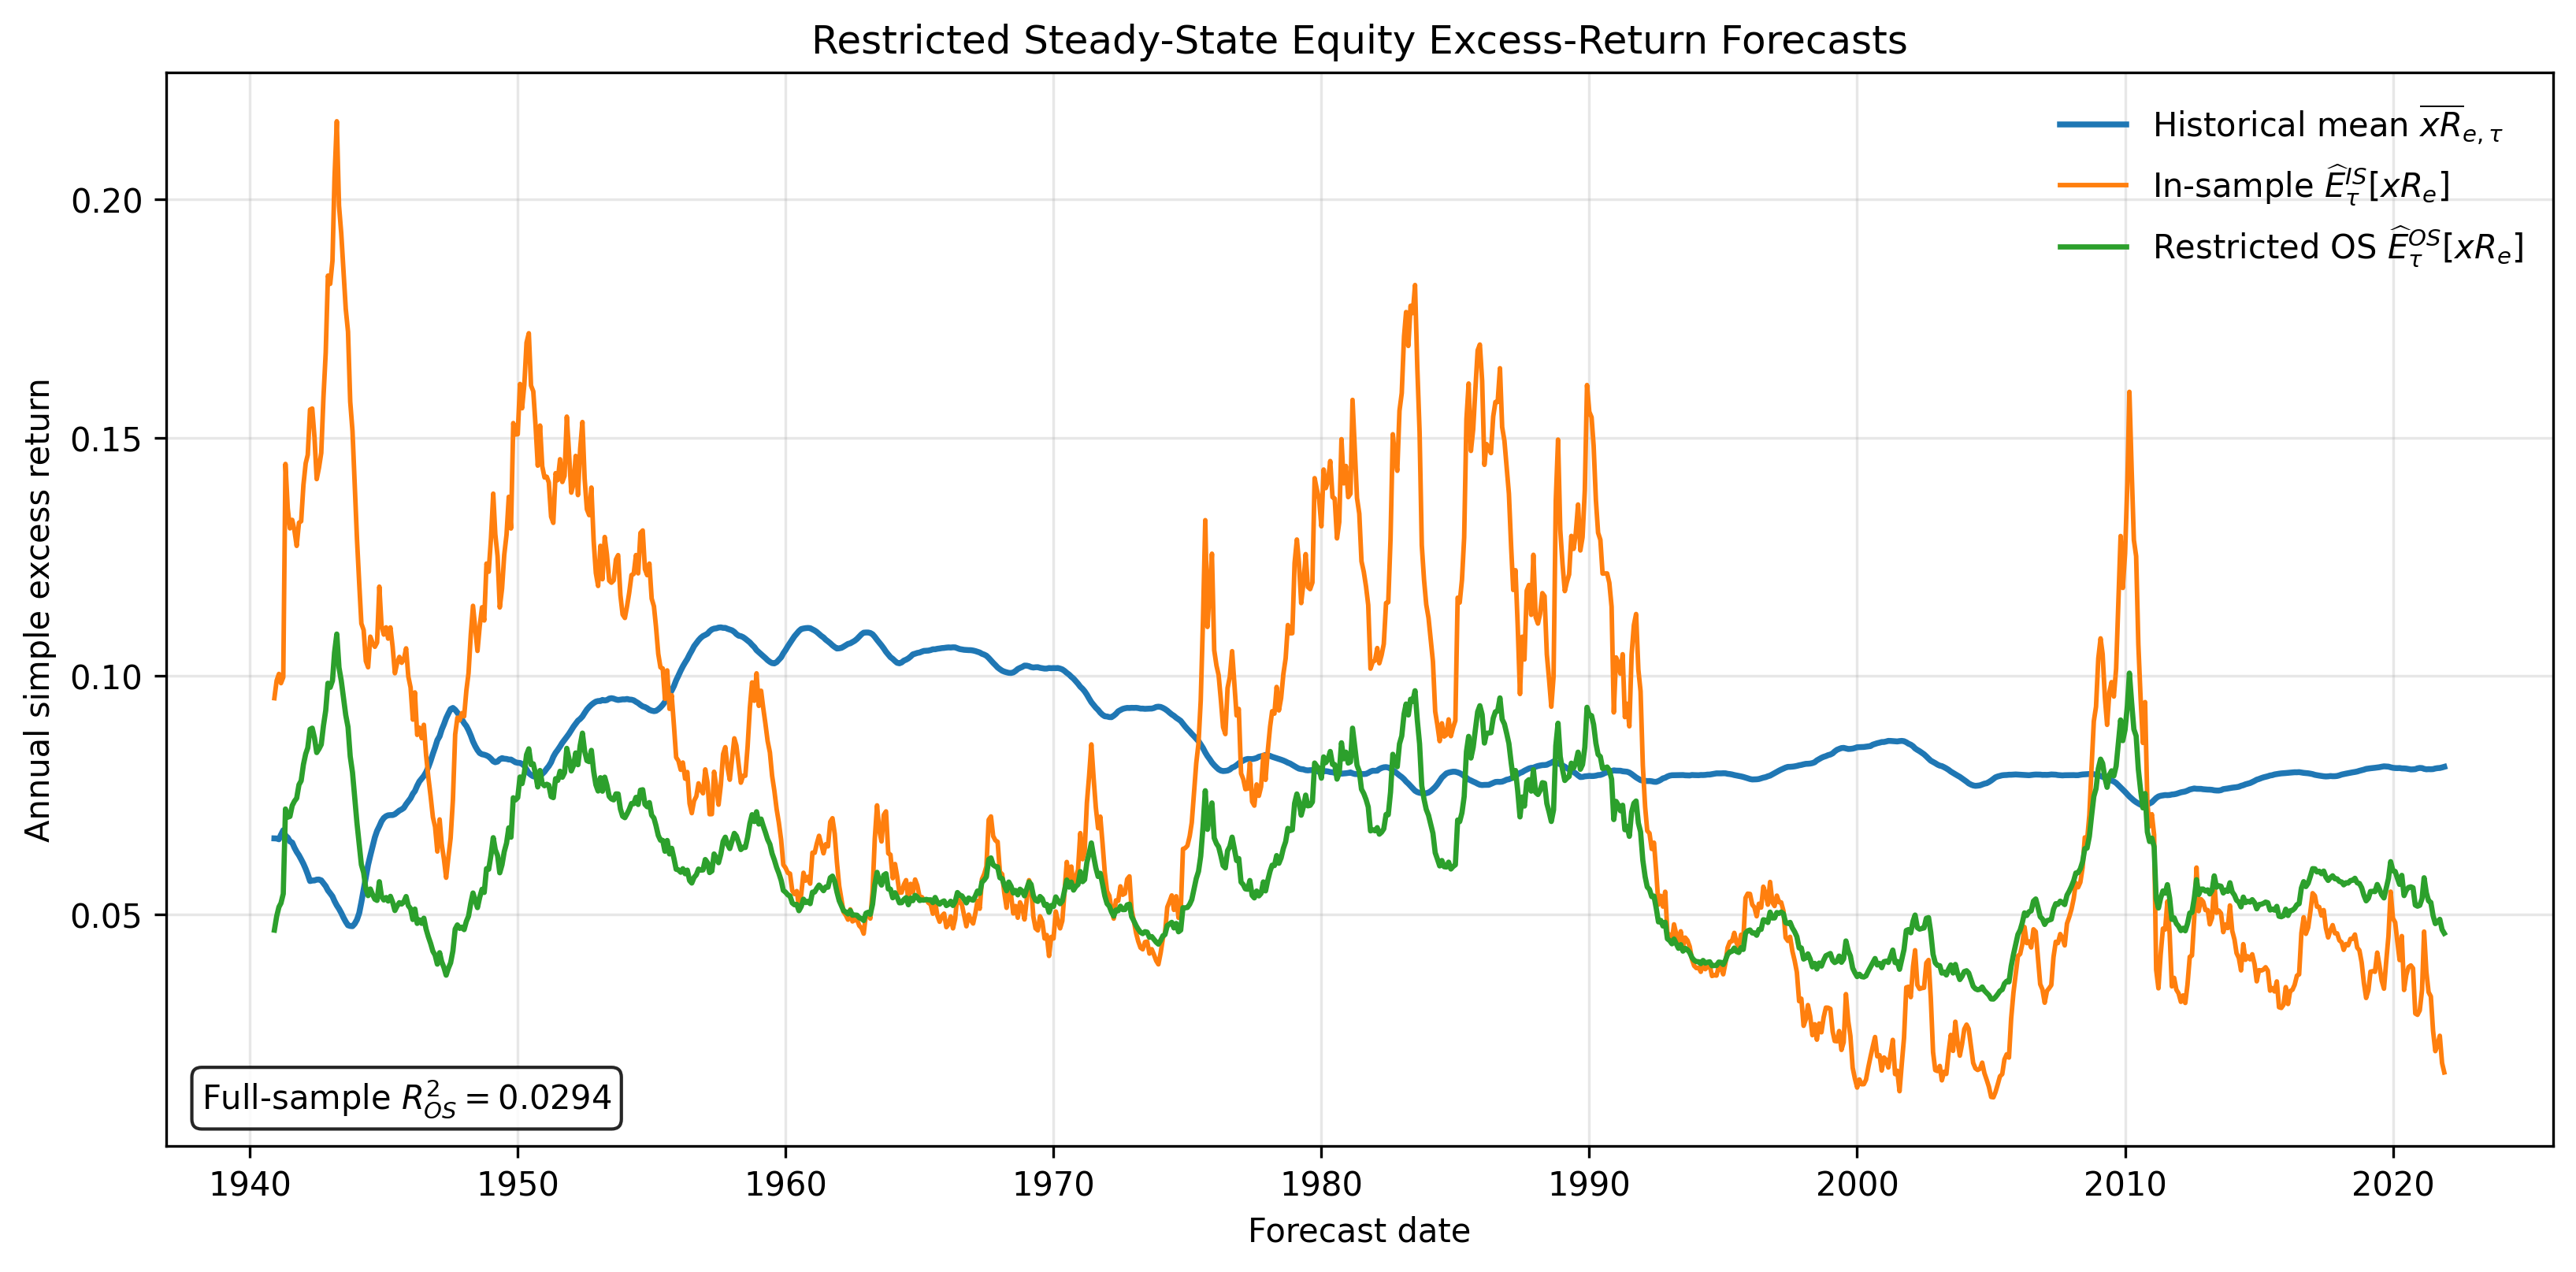
\includegraphics[width=0.9\textwidth]{figures/q2e_restricted_forecasts.png}
    \caption{Historical-mean, in-sample, and restricted steady-state
    out-of-sample forecasts of the annual simple equity excess return.}
    \label{fig:q2e_restricted_forecasts}
\end{figure}
\FloatBarrier

\begin{figure}[htbp]
    \centering
    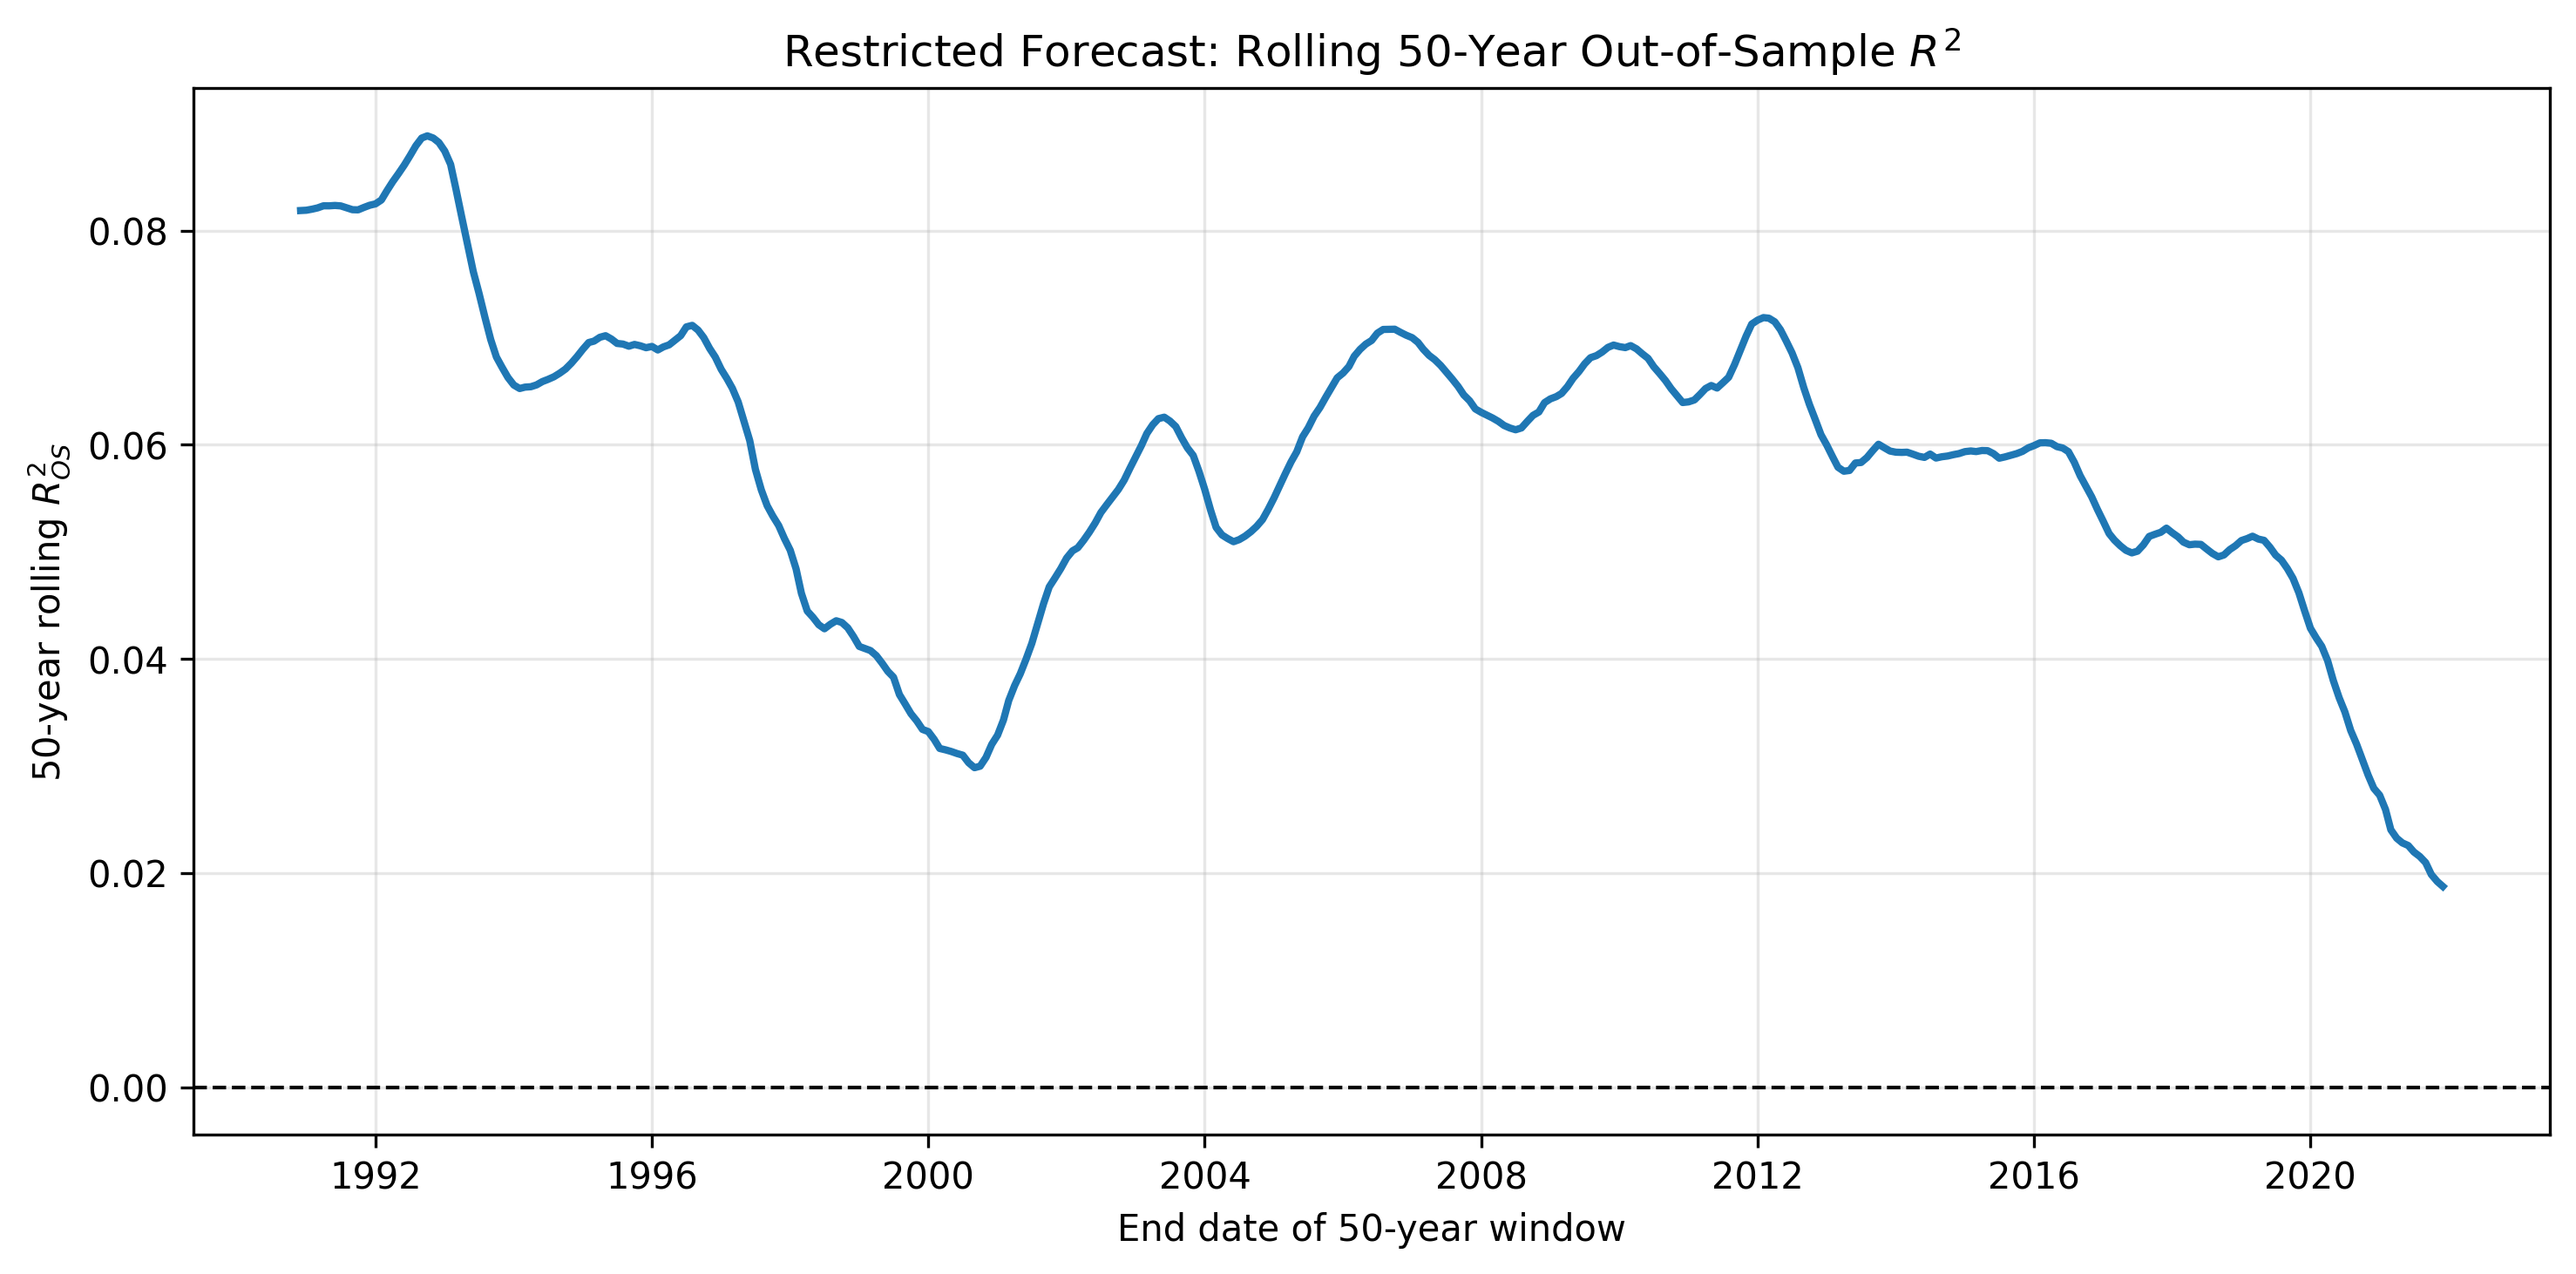
\includegraphics[width=0.9\textwidth]{figures/q2e_rolling_r2_os.png}
    \caption{Fifty-year rolling out-of-sample $R^2$ for the restricted forecast.}
    \label{fig:q2e_rolling_r2_os}
\end{figure}
\FloatBarrier
\clearpage

\section{Question 3}

% TODO

\section{Question 4}

\subsection{Part (a)}
I use the Fama--Bliss yields for maturities from one to five years. Since the original yields are reported in percentage terms, I first divide them by 100 and then construct the log yields, log forward rates, and log annual returns according to the formulas in the question. 
Because the data are monthly, I use a 12-month lag when constructing annual returns.

For each maturity $H=2,3,4,5$, I calculate the excess log yield, excess log forward rate, and excess log annual return relative to the corresponding one-year value. Table~\ref{tab:q4a_bond_averages} reports their time-series averages in percentage terms, obtained by multiplying the averages in log units by 100.

\begin{table}[htbp]
    \centering
    \caption{Time-series averages of bond excess log yields, forward rates, and annual returns (percent)}
    \label{tab:q4a_bond_averages}
    \begin{tabular}{cccc}
        \toprule
        $H$ & $\overline{xy}^{(H)}_b$ & $\overline{xf}^{(H)}_b$ & $\overline{xr}^{(H)}_b$ \\
        \midrule
        2 & 0.168613 & 0.337226 & 0.315423 \\
        3 & 0.327787 & 0.646136 & 0.606929 \\
        4 & 0.465958 & 0.880470 & 0.819825 \\
        5 & 0.563911 & 0.955723 & 0.871854 \\
        \bottomrule
    \end{tabular}
\end{table}

\end{document}
